\section{Mô phỏng}

\subsection{Mục đích và phạm vi mô phỏng}
\subsubsection{Mục đích mô phỏng}
Mục tiêu của quá trình mô phỏng là chuyển đổi mô hình giải tích trình bày ở Chương~1 thành chương trình tính toán có khả năng: (i) giải symbolic hệ ODE (\ref{eq:ode_x})--(\ref{eq:ode_y}) để thu nghiệm chính xác dạng đóng; (ii) tính toán các đại lượng đặc trưng (tầm xa, độ cao cực đại, thời gian bay) cho nhiều bộ tham số khác nhau; (iii) trực quan hóa quỹ đạo, biến thiên vận tốc và năng lượng dưới dạng đồ thị; và (iv) cung cấp giao diện tương tác cho phép thay đổi tham số và quan sát kết quả theo thời gian thực.

\subsubsection{Phạm vi và giới hạn khảo sát}
Không gian tham số được giới hạn trong các giá trị mặc định sau:
\begin{itemize}[nosep]
    \item Khối lượng $m = 1{,}0$ kg
    \item Gia tốc trọng trường $g = 9{,}81$ m/s$^2$
    \item Hệ số cản $h = 0{,}5$ kg/s (biến thiên từ 0 đến 5{,}0 trong khảo sát)
    \item Vận tốc ban đầu $v_0 = 50$ m/s
    \item Góc ném $\alpha \in \{15°, 30°, 45°, 60°, 75°\}$
    \item Thời gian khảo sát $t_{max} = 15$ s
\end{itemize}

Mô hình sử dụng lực cản tuyến tính ($F_c \propto v$), phù hợp với số Reynolds thấp. Đối với vật thể có vận tốc cao hoặc kích thước lớn ($Re \gg 1$), lực cản bậc hai ($F_c \propto v^2$) sẽ chính xác hơn; hướng mở rộng này được thảo luận tại Chương~4.

\subsection{Nền tảng công cụ và thiết kế kỹ thuật}
\subsubsection{Ngôn ngữ lập trình và thư viện}
Hệ thống mô phỏng được phát triển hoàn toàn trên \textbf{Python 3}, tận dụng hệ sinh thái thư viện khoa học phong phú. Các thư viện chính bao gồm:

\begin{itemize}[nosep]
    \item \textbf{SymPy} \cite{sympy_docs}: Tính toán symbolic -- giải hệ ODE với điều kiện ban đầu bằng hàm \texttt{dsolve()}, đơn giản hóa biểu thức, và chuyển đổi sang hàm số bằng \texttt{lambdify()}.
    \item \textbf{NumPy}: Tính toán số trên mảng đa chiều, sử dụng kỹ thuật vector hóa (vectorization) để đạt hiệu năng cao.
    \item \textbf{Matplotlib}: Vẽ đồ thị tĩnh đạt chuẩn xuất bản khoa học, xuất file ảnh PNG cho báo cáo.
    \item \textbf{Plotly}: Đồ họa tương tác (zoom, pan, hover), phục vụ phân tích trực quan trên trình duyệt.
    \item \textbf{Streamlit}: Framework xây dựng ứng dụng web tương tác, cung cấp slider, tab và các widget điều khiển mà không cần viết mã HTML/JavaScript.
\end{itemize}

\subsubsection{Kiến trúc chương trình}
Chương trình được tổ chức thành hai thành phần chính, phục vụ hai luồng công việc khác nhau:

\begin{table}[H]
\centering
\caption{Cấu trúc file chương trình}
\begin{tabular}{|l|l|p{7.5cm}|}
\hline
\textbf{File} & \textbf{Loại} & \textbf{Mô tả} \\
\hline
\texttt{projectile\_with\_drag.py} & Script tĩnh & Giải symbolic, tính toán, vẽ đồ thị Matplotlib, xuất file PNG phục vụ báo cáo \\
\hline
\texttt{app.py} & Ứng dụng Web & Giao diện Streamlit tương tác: nhập tham số bằng slider, đồ thị Plotly cập nhật theo thời gian thực \\
\hline
\end{tabular}
\end{table}

Toàn bộ mã nguồn được lưu trữ công khai tại kho GitHub:

\begin{center}
\url{https://github.com/bawfng04/VL1-Assignment}
\end{center}


\subsection{Hiện thực hóa các kịch bản mô phỏng}

\subsubsection{Giải hệ phương trình vi phân bằng SymPy}
Bước khởi đầu là thiết lập hệ ODE dưới dạng symbolic. Các biến được khai báo dưới dạng ký hiệu (symbol) của SymPy, sau đó hệ phương trình được giải bằng hàm \texttt{dsolve()} với điều kiện ban đầu tường minh.

\begin{lstlisting}[style=pythonstyle, caption={Khai báo biến symbolic và thiết lập phương trình ODE}]
from sympy import symbols, Function, Eq, dsolve, cos, sin

t = symbols('t', positive=True)
m, g, h, v0, alpha = symbols('m g h v_0 alpha', positive=True)
x = Function('x')
y = Function('y')

# Phuong trinh ODE theo phuong Ox: m*x''(t) + h*x'(t) = 0
ode_x = Eq(m * x(t).diff(t, 2) + h * x(t).diff(t), 0)

# Phuong trinh ODE theo phuong Oy: m*y''(t) + h*y'(t) = -m*g
ode_y = Eq(m * y(t).diff(t, 2) + h * y(t).diff(t), -m * g)
\end{lstlisting}

\begin{lstlisting}[style=pythonstyle, caption={Giải ODE với điều kiện ban đầu}]
# Giai phuong trinh x(t) voi dieu kien ban dau
sol_x = dsolve(ode_x, x(t), ics={
    x(0): 0,
    x(t).diff(t).subs(t, 0): v0 * cos(alpha)
})

# Giai phuong trinh y(t) voi dieu kien ban dau
sol_y = dsolve(ode_y, y(t), ics={
    y(0): 0,
    y(t).diff(t).subs(t, 0): v0 * sin(alpha)
})
\end{lstlisting}

Kết quả trả về sau khi đơn giản hóa bằng \texttt{simplify()} khớp hoàn toàn với nghiệm giải tích (\ref{eq:x})--(\ref{eq:y}) đã thiết lập ở Chương~1, xác nhận tính đúng đắn của cả hai quá trình giải.

\subsubsection{Chuyển đổi từ symbolic sang hàm số}
Biểu thức symbolic không thể trực tiếp tính toán trên mảng dữ liệu lớn. Hàm \texttt{lambdify()} của SymPy thực hiện phép chuyển đổi từ biểu thức giải tích sang hàm Python/NumPy, cho phép vector hóa tính toán:

\begin{lstlisting}[style=pythonstyle, caption={Chuyển biểu thức symbolic sang hàm số}]
from sympy import lambdify, simplify

x_expr = simplify(sol_x.rhs)
y_expr = simplify(sol_y.rhs)
vx_expr = simplify(x_expr.diff(t))
vy_expr = simplify(y_expr.diff(t))

# Chuyen sang ham so NumPy de tinh toan nhanh
params = (t, m, g, h, v0, alpha)
x_func  = lambdify(params, x_expr, 'numpy')
y_func  = lambdify(params, y_expr, 'numpy')
vx_func = lambdify(params, vx_expr, 'numpy')
vy_func = lambdify(params, vy_expr, 'numpy')
\end{lstlisting}

Sau bước này, mỗi hàm chấp nhận mảng NumPy làm đầu vào và trả về kết quả vector hóa, cho phép tính toán đồng thời trên 3000 điểm dữ liệu trong thời gian dưới 1 mili giây.

\subsubsection{Thuật toán xác định thời điểm chạm đất}
Phương trình $y(t) = 0$ với $t > 0$ không có nghiệm dạng đóng do biểu thức (\ref{eq:y}) chứa đồng thời hàm mũ và hàm tuyến tính. Thay vào đó, thời điểm chạm đất được xác định bằng phương pháp nội suy tuyến tính trên mảng dữ liệu rời rạc:

\begin{lstlisting}[style=pythonstyle, caption={Xác định thời điểm chạm đất bằng nội suy tuyến tính}]
import numpy as np

t_arr = np.linspace(0, t_max, 3000)
y_vals = y_func(t_arr, m_val, g_val, h_val, v0_val, alpha_rad)

# Tim chi so noi y chuyen dau tu duong sang am
idx = np.where((y_vals[1:] <= 0) & (y_vals[:-1] > 0))[0]
if len(idx) > 0:
    i = idx[0] + 1
    # Noi suy tuyen tinh giua hai diem lien tiep
    t_land = t_arr[i-1] + (0 - y_vals[i-1]) / \
             (y_vals[i] - y_vals[i-1]) * \
             (t_arr[i] - t_arr[i-1])
\end{lstlisting}

Sai số phương pháp bị chặn bởi $\Delta t / 2 \approx 0{,}0025$ s (với bước lưới $\Delta t = t_{max}/3000$). Đây là độ chính xác đủ cho mục đích phân tích trong bài tập lớn.

\subsubsection{Ứng dụng tương tác Web (Streamlit)}
Bên cạnh chương trình tĩnh, nhóm phát triển thêm ứng dụng web tương tác sử dụng framework Streamlit. Kiến trúc ứng dụng gồm hai phần:

\begin{itemize}[nosep]
    \item \textbf{Thanh bên (Sidebar):} Chứa các slider để nhập trực tiếp giá trị $m$, $g$, $h$, $v_0$, $t_{max}$ và chọn góc ném $\alpha$ theo ba chế độ: tập góc cố định, slider tùy chỉnh, hoặc nhập tự do.
    \item \textbf{Khu vực chính:} Hiển thị 6 tab phân tích, mỗi tab tự động cập nhật khi tham số thay đổi.
\end{itemize}

\begin{table}[H]
\centering
\caption{Các tab chức năng trong ứng dụng Streamlit}
\begin{tabularx}{\textwidth}{|l|X|}
\hline
\textbf{Tab} & \textbf{Chức năng} \\
\hline
Quỹ đạo & Vẽ quỹ đạo $y(x)$ cho các góc đã chọn, kèm bảng số liệu chi tiết \\
\hline
So sánh lực cản & So sánh quỹ đạo có và không có lực cản, tính chênh lệch $\Delta R$ và $\Delta H$ \\
\hline
Vận tốc & Đồ thị $v_x(t)$, $v_y(t)$, $|v|(t)$ trên 3 panel riêng biệt \\
\hline
Năng lượng & Biến thiên động năng, thế năng, cơ năng, và năng lượng tiêu hao do cản \\
\hline
Khảo sát $h$ & Khảo sát ảnh hưởng của hệ số cản đến quỹ đạo với phạm vi tùy chỉnh \\
\hline
Lý thuyết & Trình bày phương trình Newton II, nghiệm giải tích, nhận xét vật lý \\
\hline
\end{tabularx}
\end{table}

Một điểm kỹ thuật đáng lưu ý: hàm giải ODE symbolic được đánh dấu \texttt{@st.cache\_resource} thay vì \texttt{@st.cache\_data}, do các đối tượng \texttt{lambdify} không hỗ trợ serialize bằng \texttt{pickle}. Decorator \texttt{cache\_resource} cho phép lưu trữ tham chiếu trực tiếp đến đối tượng trong bộ nhớ mà không cần serialize, đảm bảo hàm giải chỉ chạy một lần duy nhất.

\textbf{Hướng dẫn cài đặt và chạy ứng dụng:}
\begin{lstlisting}[style=pythonstyle, caption={Lệnh cài đặt và khởi chạy ứng dụng}, language=bash]
# Cai dat cac thu vien phu thuoc
pip install -r requirements.txt

# Khoi chay ung dung
streamlit run app.py
\end{lstlisting}

Ứng dụng tự động mở trình duyệt tại \texttt{http://localhost:8501}. 

\subsubsection{Giao diện ứng dụng tương tác}
Các hình dưới đây minh họa giao diện ứng dụng khi vận hành với bộ tham số mặc định.

\begin{figure}[H]
\centering
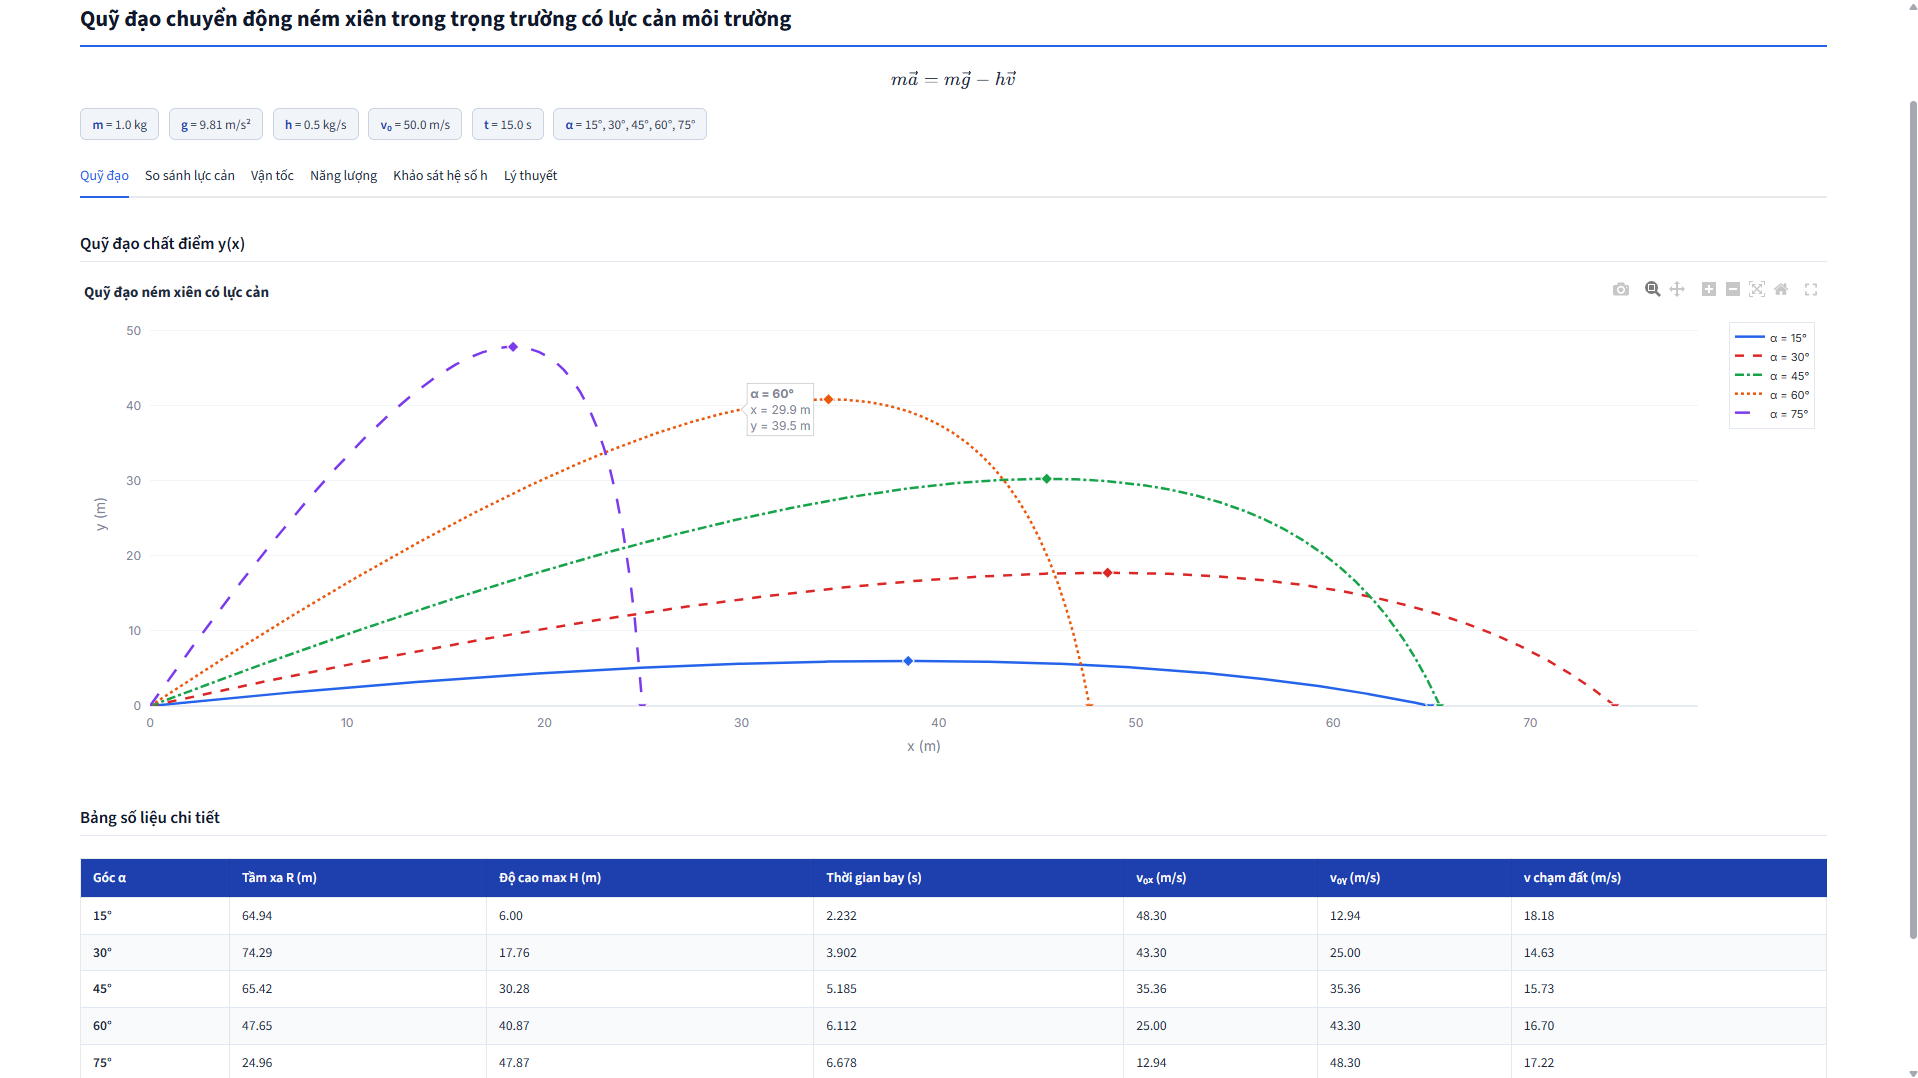
\includegraphics[width=\textwidth]{images/ss01.png}
\caption{Tab ``Quỹ đạo'': quỹ đạo $y(x)$ cho 5 góc ném kèm bảng số liệu. Các tham số vật lý hiển thị dưới dạng thẻ (chip) ngay phía trên đồ thị.}
\label{fig:ss01}
\end{figure}

\begin{figure}[H]
\centering
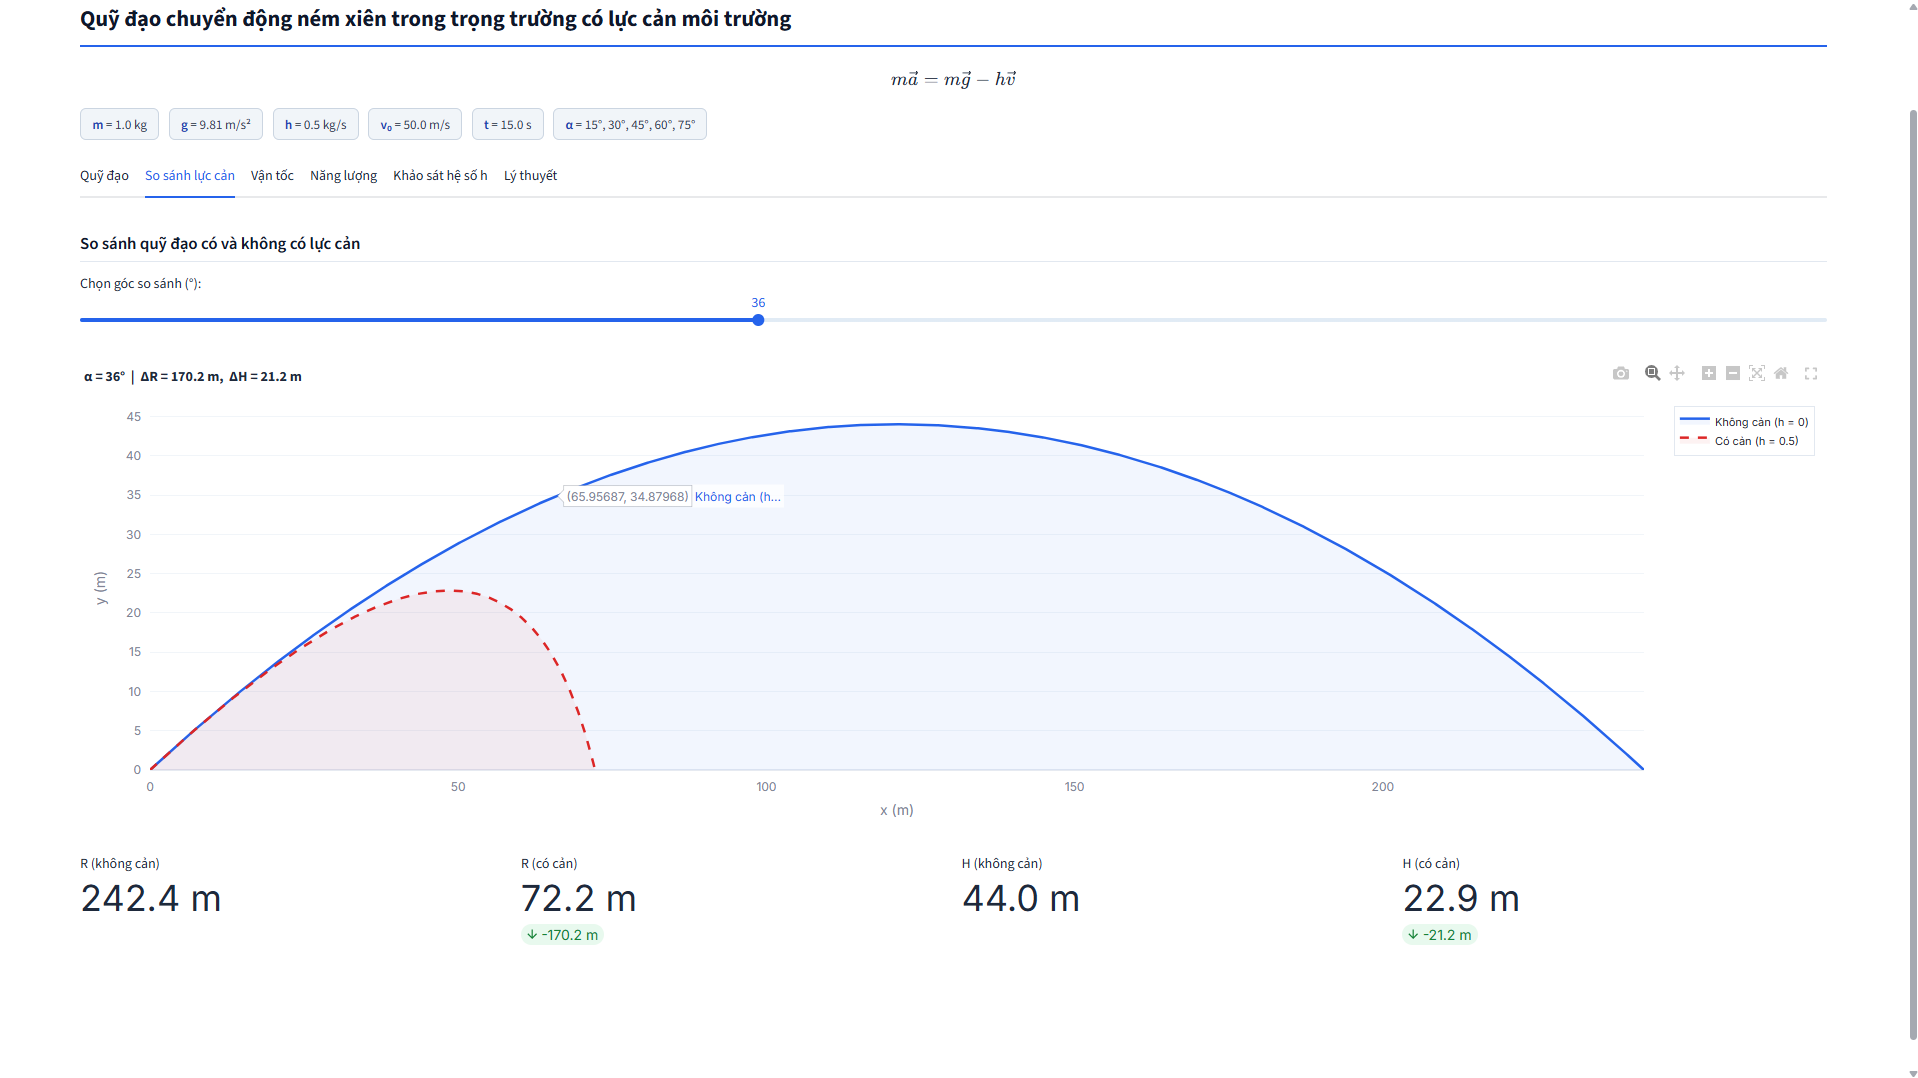
\includegraphics[width=\textwidth]{images/ss02.png}
\caption{Tab ``So sánh lực cản'': thanh trượt cho phép chọn góc $\alpha = 36°$. Sự chênh lệch $\Delta R$ và $\Delta H$ giữa hai trường hợp được tính và hiển thị tự động.}
\label{fig:ss02}
\end{figure}

\begin{figure}[H]
\centering
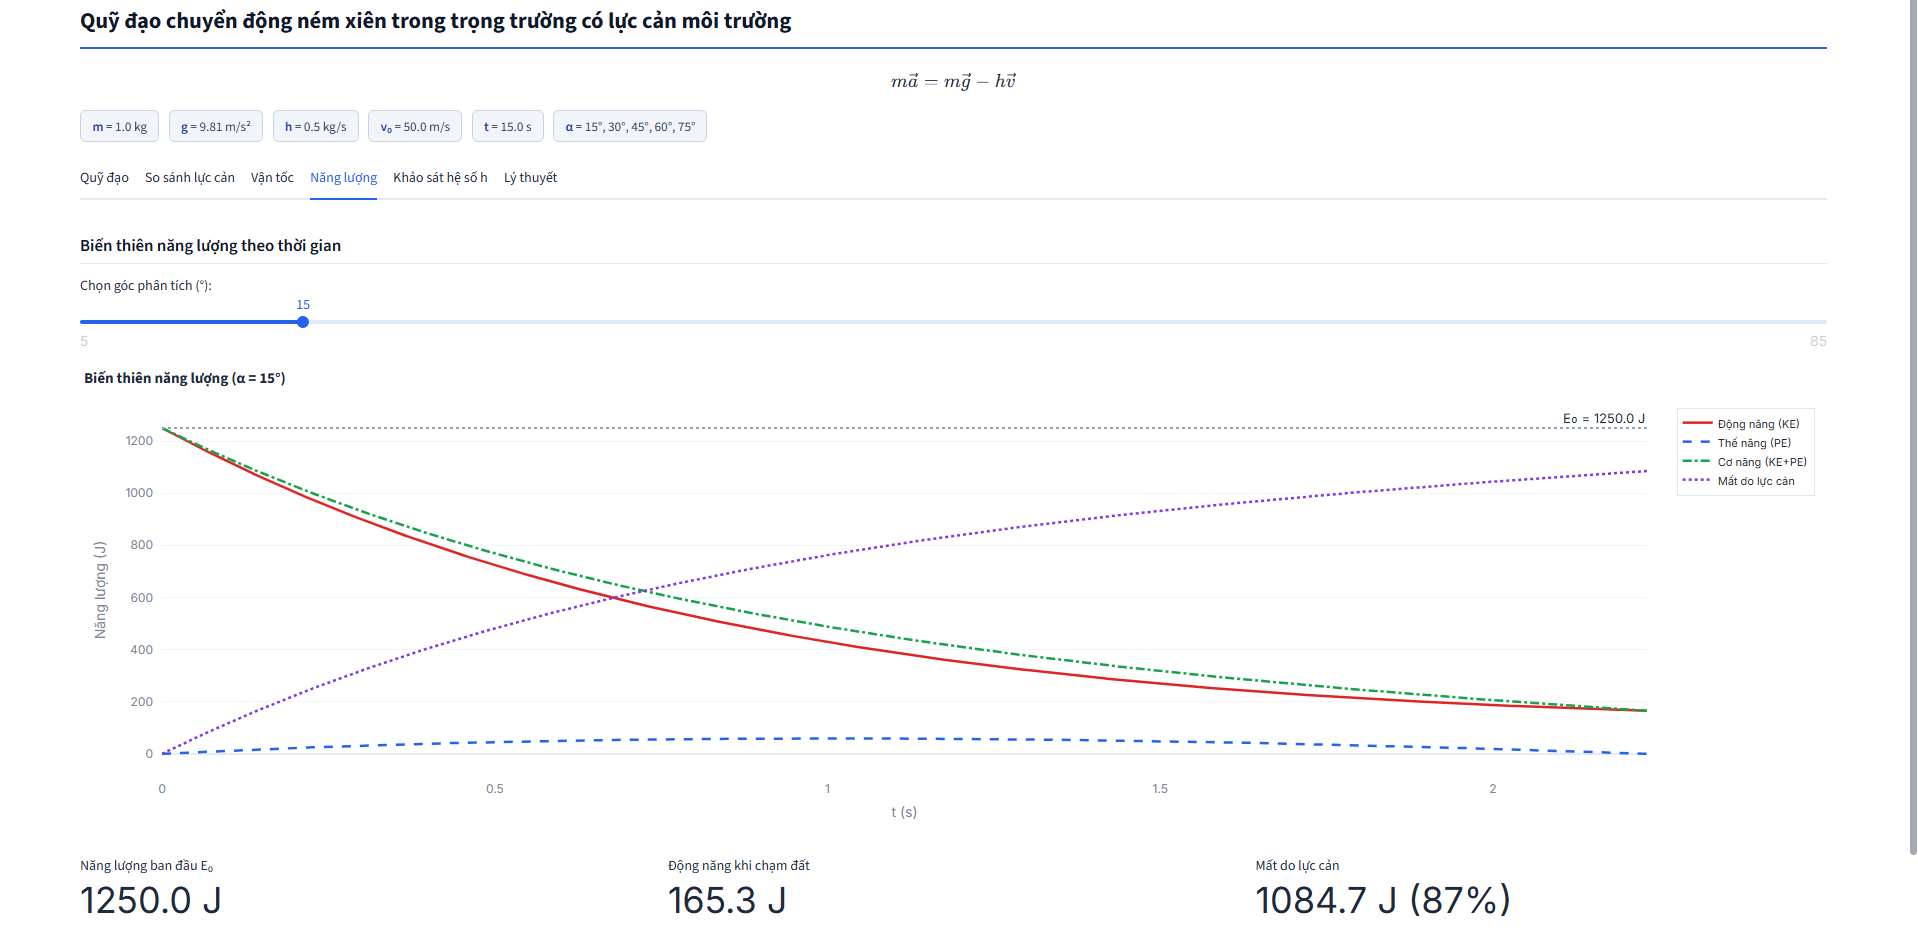
\includegraphics[width=\textwidth]{images/ss04.png}
\caption{Tab ``Năng lượng'': phân tích biến thiên năng lượng tại góc $\alpha = 15°$. 87\% năng lượng ban đầu bị tiêu hao do lực cản. Các chỉ số tổng hợp hiển thị phía dưới đồ thị.}
\label{fig:ss04}
\end{figure}
